% !TEX encoding = UTF-8 Unicode
% !TEX root = thesis.tex


%\section{Markerless Motion Capture\\with Frankenstein's Model}
\section{Motion Capture with Frank}

We fit the Frank model to data to capture the total body motion, including the major limbs, the face, and fingers. Our motion capture method relies heavily on fitting mesh correspondences to 3D keypoints, which are obtained by triangulation of 2D keypoint detections across multiple camera views. To capture shape information we also use point clouds generated by multiview stereo reconstructions. Model fitting is performed by an optimization framework to minimize distances between corresponded model joints and surface points and 3D keypoint detections, and iterative closest point (ICP) to the 3D point cloud. Note that more details are provided in the supplementary material.
% In total we reconstruct XX 3D keypoints. 

\subsection{3D Measurements}
\label{subsection:landmark_reconstruction}
We incorporate two types of measurements in our framework as shown in Fig.~\ref{fig:3dlandmarks_model_fitting}: (1) corresponded 3D keypoints, which map to known joints or surface points on the mesh models (see Fig.~\ref{fig:frankenstein_part_aligned}), and (2) uncorresponded 3D points from multiview stereo reconstruction, which we match using ICP. 
% All measurements are obtained for each frame independently, but keypoints from a same individual across time are associated by considering thresholding the distance of a facial keypoint between frames.


\textbf{3D Body, Face, and Hand Keypoints:}  We use the OpenPose detector~\cite{openpose} in each available view, which produces 2D keypoints on the body with the method of Cao et al.~\cite{cao2017realtime}, and hand and face keypoints using the method of Simon et al.~\cite{simon2017hand}. 3D body skeletons are obtained from the 2D detections using the method of~\cite{joo2017panoptic}, which uses known camera calibration parameters for reconstruction. The 3D hand keypoints are obtained by triangulating 2D hand pose detections, following the method of \cite{simon2017hand}, and similarly for the facial keypoints. Note that subsets of 3D keypoints can be entirely missing if there are not enough 2D detections for triangulation, which can happen in challenging scenes with inter-occlusions or motion blur. 

\textbf{3D Feet Keypoints:} An important cue missing from the OpenPose detector is keypoints on the feet. For motion capture, this is an essential feature to accurately determine the orientation of the feet. We therefore train a keypoint detector for the tip of the big toe, the tip of the little toe, and the ball of the foot. We annotate these 3 keypoints per foot in each of around 5000 person instances of the COCO dataset, and use the architecture of Wei et al.~\cite{Wei2016} with a bounding box around the feet determined by the 3D body detections. We also apply multiview bootstrapping in the Panoptic Studio to improve the quality, as described by Simon et al.~\cite{simon2017hand}.%\footnote{More details provided in the supplementary material.}.

%The detector is improved multiview bootstrap in the Panoptic Studio Data. In testing time, bounding box is obtained by projecting the 3D ankle keypoints of the body reconstruction, providing the association between body and feet by construction. 

%
%\textbf{Discussion:} The 3D landmark reconstruction is done per-frame and it is free from error accumulation or other assumption about the scene. More importantly, it works on face and hand even if the limited resolution, which was not possible by directly reconstruction from views. 
%
%This results provide a crucial information to temporally align the pose in the canonical data for fusion the geometry information.
%
%However, the method typically suffers from jitter, and sometime produce noticiabllly wrong result since it doens't have any contraint about bone length and temporal coherency.  And the parts are missing if detection is failed. 

\textbf{3D Point Clouds:} We use the commercial software RealityCapture~\cite{RealityCapture} to obtain 3D point clouds from the multiview images, with associated point normals.

% \begin{figure}[t]	
% 	%	\includegraphics[width=0.24\columnwidth,trim=900 110 1000 90, clip]{fig/landmarks/skeleton_original}	\llap{\frame{ {\includegraphics[width=0.8cm,trim=1100 1100 1200 200, clip]{fig/landmarks/skel_sub}}}}
% 	\includegraphics[width=0.24\columnwidth,trim=900 110 1000 90, clip]{fig/landmarks/skeleton_original}
% 	\includegraphics[width=0.24\columnwidth,trim=900 110 1000 90, clip]{fig/landmarks/surface}	
% 	\includegraphics[width=0.24\columnwidth,trim=900 110 1000 90, clip]{fig/landmarks/skel_mesh}
% 	\includegraphics[width=0.24\columnwidth,trim=900 110 1000 90, clip]{fig/landmarks/mesh}	
	
% 	\caption{3D measurements and a Frankenstein Model fitting result. (a) 3D keypoints from body, face, hands, and feet. The face has additional keypoints (ears, pupils and nose), which are not displayed in this figure; (b) 3D point clouds reconstructed from 31 HD cameras; (3 and 4) Frankenstein Model fitting results}
% 	\label{fig:3dlandmarks_model_fitting}
% \end{figure}

\begin{figure}[t]	
	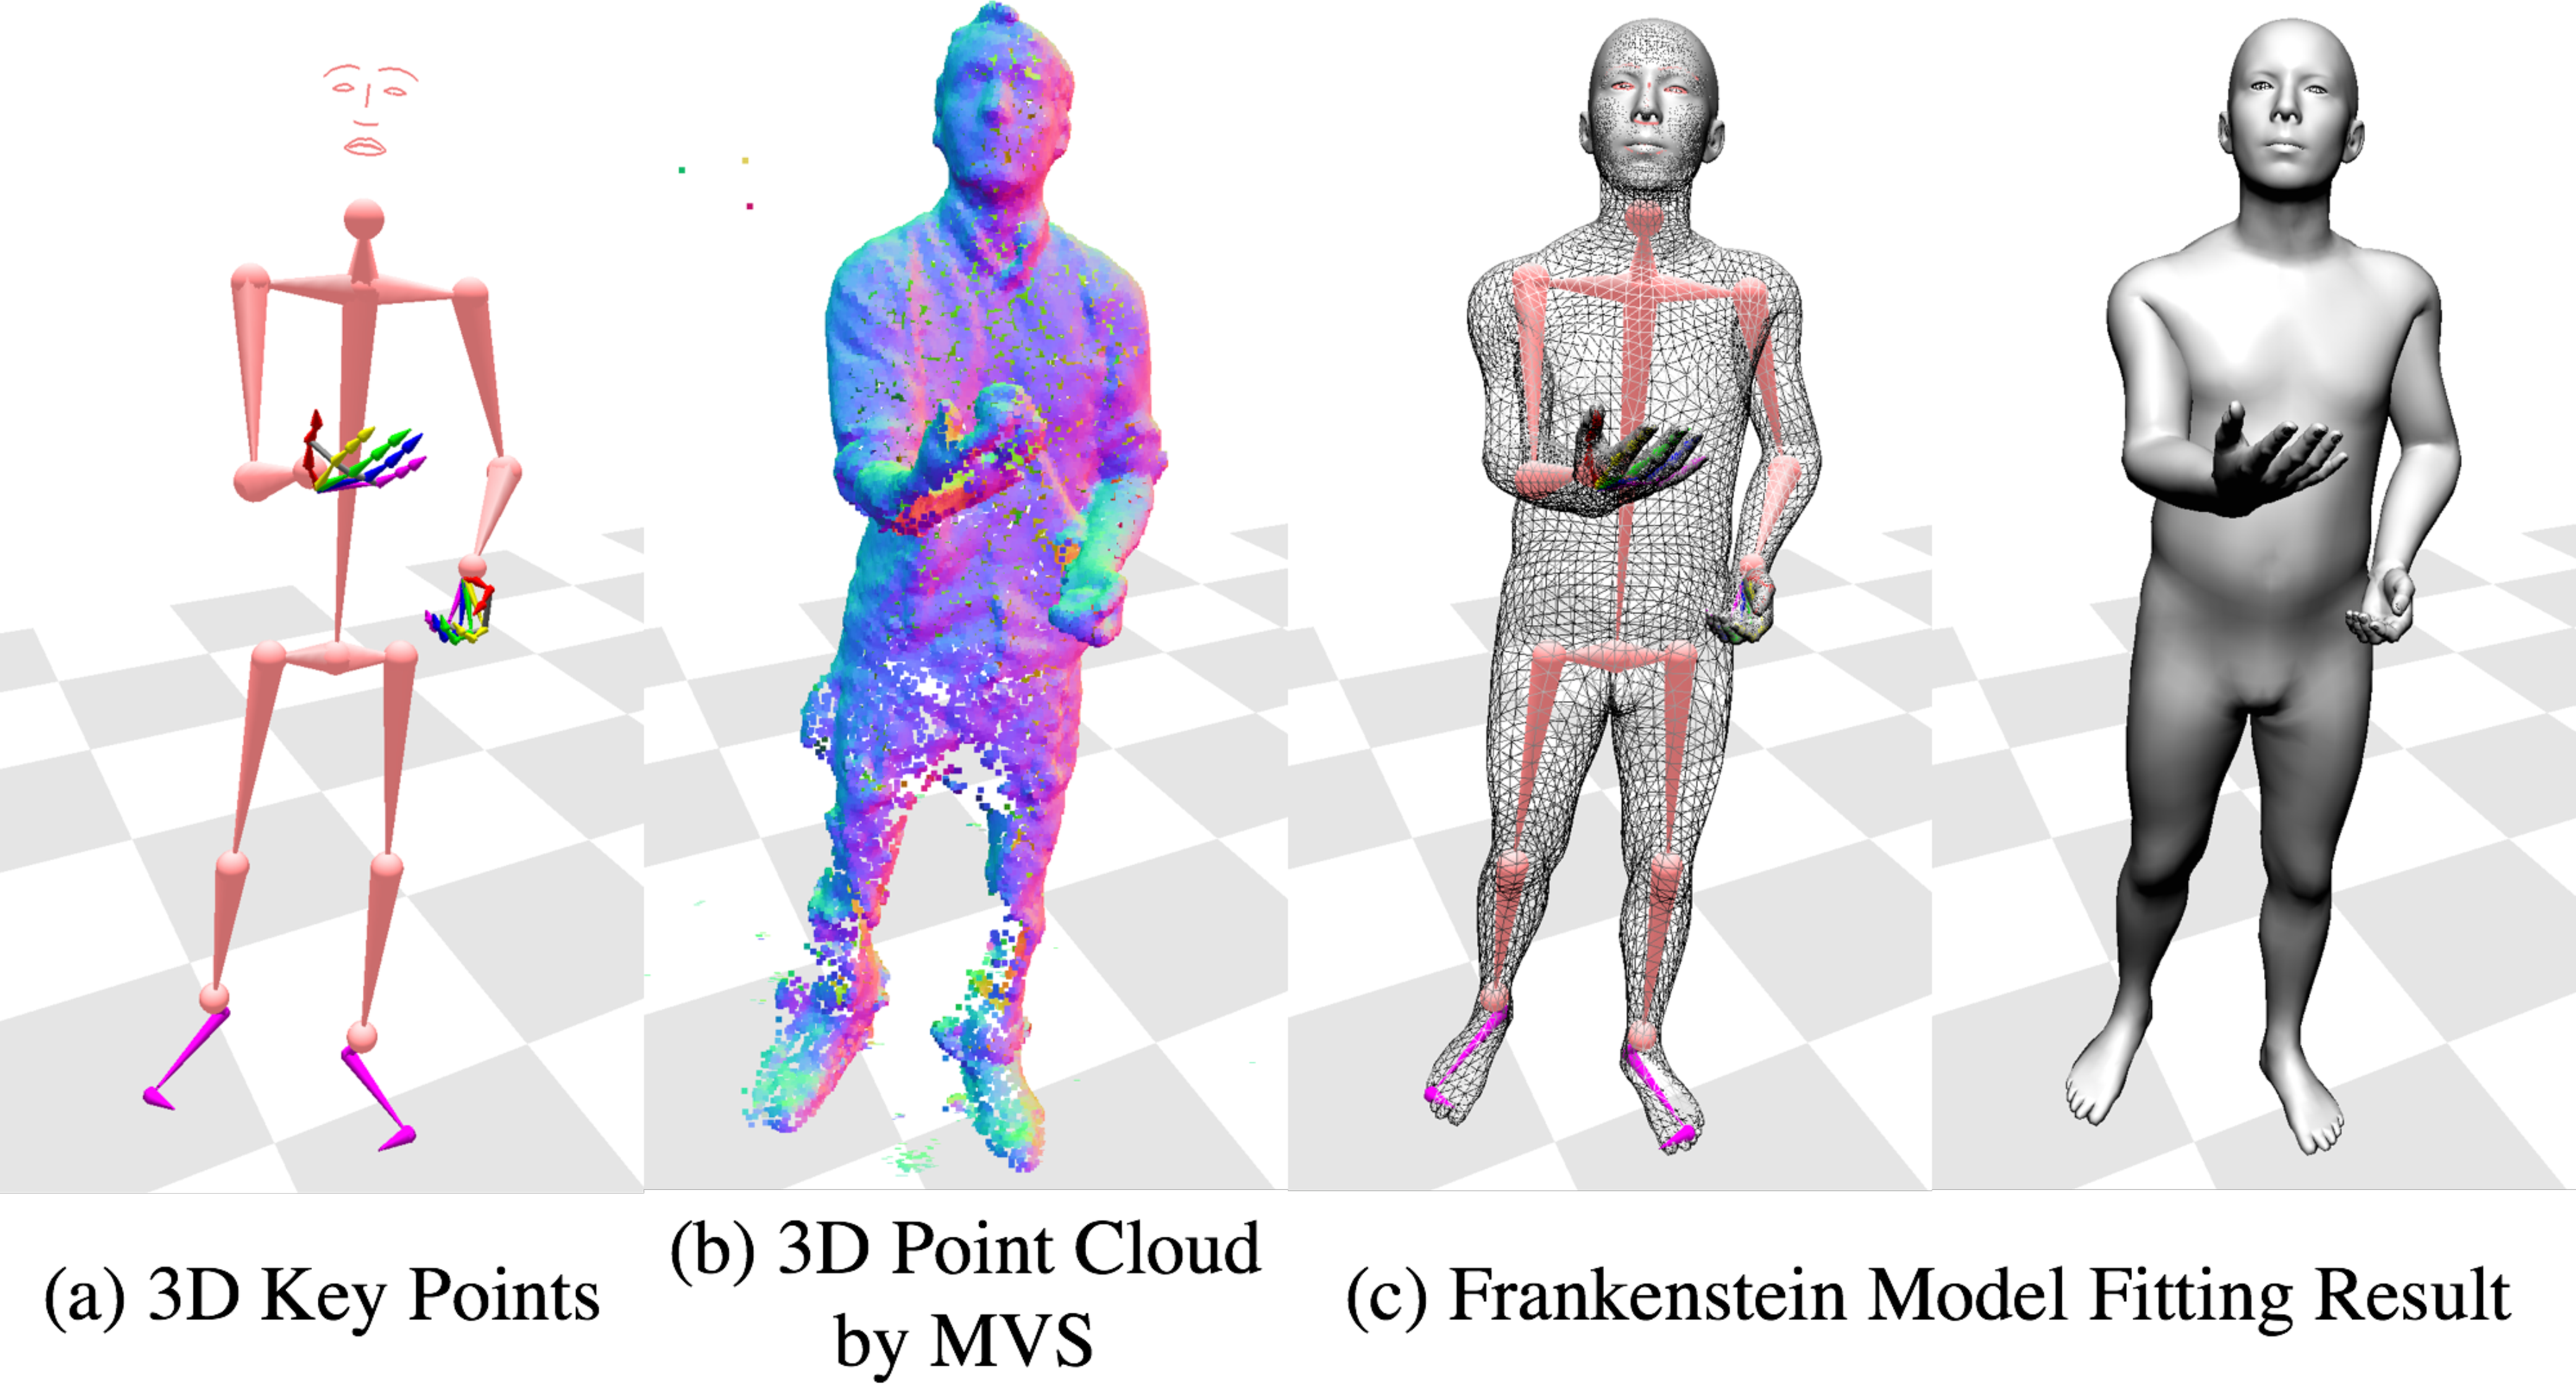
\includegraphics[width=\columnwidth]{tbc_figures/3Dmeasurements_legend2}
	\caption{Fitting Frank: The optimization takes, as input, (a) 3D keypoints, and (b) point clouds, and produces (c) a fitted skeleton and mesh as output.}
	\label{fig:3dlandmarks_model_fitting}
\end{figure}

%\begin{figure}[t]
%	\includegraphics[width=\columnwidth]{fig/modelAlignment}		\includegraphics[width=\columnwidth]{fig/modelAlignment2}
%	
%	\caption{Template model alignment to pre-compute correspondences}
%	\label{fig:modelAlignment}
%\end{figure}
%

%
%\subsection{Full Body Model}
%To recap, the full body model is parameterized by the following variables, which define the final position of each of the model's vertices in world coordinates:
%\begin{center}
%	\begin{tabular}{|c|c|c|} \hline 
%		Symbol & Meaning & Size \\ \hline\hline
%		$\mathbf{a}$ & Body shape coefficients & $10$\\ \hline
%		$\boldsymbol{\theta}$ & Body pose & $3\times 24$\\ \hline
%		$\mathbf{c}$ & Face shape coefficients & $150$ \\ \hline
%		$\mathbf{e}$ & Facial expression coefficients & $200$ \\ \hline
%		$\boldsymbol{\phi}^r$ & Right hand pose & $3\times 16$ \\ \hline
%		$\boldsymbol{\phi}^l$ & Left hand pose & $3\times 16$ \\ \hline
%		$\boldsymbol{s}$ & Hand scale parameters & $3\times 16$ \\ \hline
%		$\boldsymbol{t}$ & Global translation & $3$ \\ \hline
%		\hline
%	\end{tabular}
%\end{center}
%While the number of facial coefficients is larger than the degrees of freedom of other parts of the body, it should be noted that these parameters are heavily constrained by a prior, and, in fact, almost all of the variation in the training set is captured within approximately the first 60 coefficients. 
%
%Conceptually, the parameter set can be split into two categories. One set of parameters are static shape or {\em identity} parameters, including body shape, face shape, and hand scaling factors, which do not vary with time (e.g., bone lengths): 
%\begin{align}
%\mathcal{S} = \{\mathbf{a}, \mathbf{c}, \mathbf{s} \}.
%\end{align}
%The remaining parameters are per-frame {\em expression} parameters, including body pose, hand pose, facial expression, and global orientation and translation, 
%\begin{align}
%\mathcal{E}_t = \{ \boldsymbol{\theta}_t, \mathbf{e}_t, \boldsymbol{\phi}^r_t, \boldsymbol{\phi}^l_t,  \mathbf{t}_t \}.
%\end{align}
%This set of parameters is inherently dynamic and we index it with the sub-index $t$ to indicate that they are time-varying. To simplify the exposition, we will abstract away the details of each of the models used and instead denote the concatenated set of vertices,
%\begin{align}
%\mathbf{V}_t = [ \mathbf{V}_b, \mathbf{V}_f, \mathbf{V}_{hr}, \mathbf{V}_{hl} ] = B( \mathcal{S}, \mathcal{E}_t ),
%\end{align}
%where $\mathbf{V}_t\in\mathds{R}^{3\times V}$ with $V$ the total number of vertices, and the function $B(\cdot)$ maps from the combined model parameters, including static and per-frame parameters, to the full configuration of vertices for the body, face, and hands.

\subsection{Objective Function}

We initially fit every frame in the sequence independently. For clarity, we drop the time index from the notation and describe the process for a single frame, which optimizes the following cost function:
\begin{align}
\label{eq:fitting_franken}
E\big( \boldsymbol{\theta}^U, \boldsymbol{\phi}^U, \boldsymbol{t}^U \big) = E_\textrm{keypoints} + E_\textrm{icp} + E_\textrm{seam} +E_\textrm{prior}
\end{align}
We use Levenberg-Marquardt with the Ceres Solver library~\cite{ceres-solver} with multiple stages to avoid local minima. See the supplementary material for the details.

\textbf{Anatomical Keypoint Cost:} The term $E_\textrm{keypoints}$ matches 3D keypoint detections, which are in direct corresponce to our mesh models. This term includes joints (or end effectors) in the body and hands, and also contains points corresponding to the surface of the mesh (e.g., facial keypoints and the tips of fingers and toes). Both of these types of correspondence are expressed as combinations of vertices via a regression matrix $\mathbf{J}\,{\in}\,\mathds{R}^{C\times N^U}$, where $C$ denotes the number of correspondences and $N^U$ is the number of vertices in the model. Let $\mathcal{D}$ denote the set of available detections in a particular frame. The cost is then:
%We denote the aggregation of all 3D keypoints at time $t$ as $\mathbf{Y}_t$ and denote the aggregation of all corresponding joints and surface vertices as $\mathbf{V}_t$
\begin{align}
E_\textrm{keypoints} = \lambda_\textrm{keypoints} \sum_{i\in\mathcal{D}}|| \mathbf{J}_i \mathbf{V} - \mathbf{y}_i^T ||^2,
\label{eq:detection_eq}
\end{align}
where $\mathbf{J}_i$ indexes a row in the correspondence regression matrix and represents an interpolated position using a small number of vertices, and $\mathbf{y}_i\,{\in}\,\mathds{R}^{3 \times 1}$ is the 3D detection. The $\lambda_\textrm{keypoints}$ is a relative weight for this term.

\textbf{ICP Cost:} The 3D point cloud measurements are not a priori in correspondence with the model meshes. We therefore establish their correspondence to the mesh using Iterative Closest Point (ICP) during each solver iteration. 
We find the closest 3D point in the point cloud to each of the mesh vertices, and compute the point-to-plane residual, i.e., the distance along the normal direction,
\begin{align}
E_\textrm{icp} = \lambda_\textrm{icp} \sum_{\mathbf{v}_j \in \mathbf{V}^U} \mathbf{n}(\mathbf{x}_{j^*})^T (\mathbf{x}_{j^*} - \mathbf{v}_j ),
\end{align}
where $\mathbf{x}_{i^*}$ is the closest 3D point to $j$-th vertex $\mathbf{v}_j$,  $\mathbf{n}(\cdot)\in\mathds{R}^3$ represents the point's normal, and $\lambda_\textrm{icp}$ is a relative weight for this term. 
%Some details

%
%\begin{align}
%i^*= \operatorname{arg} \operatorname{min}_i  || \mathbf{x}_i - \mathbf{v}_j ||^2,
%\end{align}
%where $\mathbf{x}_{i^*}$ is the closest 3D point to vertex $j$, where $\mathbf{v}_j$ is a vertex\footnote{We do not consider some parts (around hands and face), as depth sensor resolution is too low to improve the estimate. These parts are excluded by a mask.} in $\mathbf{V}^U$ of the Frank model. To ensure that this is a correct correspondence, we use thresholds for the distance and normals during the correspondence search.
%
%Finally, for each vertex~$j$ we compute the point-to-plane residual, i.e., the distance along the normal direction,
%\begin{align}
%E_\textrm{icp} = \lambda_\textrm{icp} \sum_{\mathbf{v}_j \in \mathbf{V}^U_t} \mathbf{n}(\mathbf{x}_{i^*})^T (\mathbf{x}_{i^*} - \mathbf{v}_j ),
%\end{align}
%where $\mathbf{n}(\cdot)\in\mathds{R}^3$ represents the point's normal, and $\lambda_\textrm{icp}$ is a relative weight for this term. 

\textbf{Seam Constraints:} The part models composing the Frank model are rigidly linked by the skeletal hierarchy. However, the independent surface parameterizations of each of the part models may introduce discontinuities at the boundary between parts (e.g., a fat arm with a thin wrist). To avoid this artifact, we encourage the vertices around the seam parts to be close by penalizing differences between the last two rings of vertices around the seam of each part, and the corresponding closest point in the body model in the rest pose expressed as barycentric coordinates. %See the supplementary materials for details.
% with $\mathbf{B}_i\,{\in}\,\mathds{R}^{1\times N^B}$ (where $\mathbf{B}_i\mathbf{1}_{N^B}{=}1$), and similarly for the right hand and face.
%\begin{align}
%E_\textrm{seam} = &|| \mathbf{V}_{lh:B} - \mathbf{Y}_{B:lh} ||^2 +\\
% &|| \mathbf{V}_{rh:B} - \mathbf{Y}_{B:rh} ||^2 +\\
%  &|| \mathbf{V}_{F:B} - \mathbf{Y}_{B:F} ||^2,
%\label{eq:glue_constraints}
%\end{align}
%
% \begin{align}
% E_\textrm{seam} = &\sum_{(i,j)\in\mathcal{C}^{LH}} || \mathbf{B}_i\mathbf{V}^B - (\mathbf{v}^{LH}_{j})^T ||^2 +\\
%  &\sum_{(i,j)\in\mathcal{C}^{RH}} || \mathbf{B}_i \mathbf{V}^B - (\mathbf{v}^{RH}_{j})^T ||^2 +\\
%   &\sum_{(i,j)\in\mathcal{C}^{B}} || \mathbf{B}_i \mathbf{V}^B - (\mathbf{v}^{F}_{j})^T ||^2,
% \label{eq:glue_constraints}
% \end{align}
%\begin{align}
%E_\textrm{glue} = &\sum_{(i,j)\in\mathcal{C}^{LH}} || \mathbf{v}^B_{i} - \mathbf{v}^{LH}_{j} ||^2 +\\
% &\sum_{(i,j)\in\mathcal{C}^{RH}} || \mathbf{v}^B_{i} - \mathbf{v}^{RH}_{j} ||^2 +\\
%  &\sum_{(i,j)\in\mathcal{C}^{B}} || \mathbf{v}^B_{i} - \mathbf{v}^{F}_{j} ||^2,
%\label{eq:glue_constraints}
%\end{align}
% where the set $\mathcal{C}^{LH}$ contains correspondences $(i,j)$ where $j$ indexes the last two rings of vertices around the seam of the left hand, and $i$ denotes the corresponding closest point in the body model in the rest pose expressed as barycentric coordinates with $\mathbf{B}_i\,{\in}\,\mathds{R}^{1\times N^B}$ (where $\mathbf{B}_i\mathbf{1}_{N^B}{=}1$), and similarly for the right hand and face.

\textbf{Prior Cost:} 
Depending on the number of measurements available in a particular frame, the set of parameters of $M^U$ may not be determined uniquely (e.g., the width of the fingers). More importantly, the 3D point clouds are noisy and cannot be well explained by the model due to hair and clothing, which are not captured by the SMPL and FaceWarehouse meshes, resulting in erroneous correspondences during ICP. Additionally, the joint locations of the models are not necessarily consistent with the annotation criteria used to train the 2D detectors. We are therefore forced to set priors over model parameters to avoid the model from overfitting to these sources of noise, $E_\textrm{prior} = E^F_\textrm{prior} + E^B_\textrm{prior} + E^H_\textrm{prior}$.
% \begin{align}
% E_\textrm{prior} = E^F_\textrm{prior} + E^B_\textrm{prior} + E^H_\textrm{prior}
% \end{align}
The prior for each part is defined by corresponding shape and pose priors, for which we use zero-mean standard normal priors for each parameter except for scaling factors, which are encouraged to be close to 1. %Details and relative weights can be found in supplementary materials.
% All PCA derived parameters are penalized with the corresponding variance, which by construction 

% of our basis is:
% \begin{align}
% E_\textrm{prior}^F &= \lambda_{SF} ||\phi^F||^2 + \lambda_{PF} ||\theta^F||^2\\
% E_\textrm{prior}^B &= \lambda_{SB} ||\phi^B||^2 + \lambda_{PB} ||\theta^B||^2\\
% E_\textrm{prior}^H &= \lambda_{SH} ||\phi^H-1||^2 + \lambda_{PH} ||\theta^H||^2
% \end{align}
% where, for simplicity, we penalize pose parameters that deviate from the rest pose with a small weight, and we encourage hand scaling factors to be close to 1.
%\begin{align}
%E_\textrm{prior}^F = E^F_\textrm{prior}(\phi^F) + E^F_\textrm{prior}(\theta^F)\\
%E^F_\textrm{prior}(\phi^F) = {\phi^F}^T\phi^F\\
%E^F_\textrm{prior}(\theta^F) = {\theta^F}^T\theta^F,
%\end{align}
% and similarly for other part model parameters. We use different weights for the priors on different parts ($\lambda_{SF}=\lambda_{SH}=10^{-2}$, $\lambda_{SB}=10^{-2}, \lambda_{PF}=10^{-4}, \lambda_{PB}=10^{-6}$, and $\lambda_{PH}=10^{-7}$).

%face_shape 1e-4
%body shape 1e-2
%hand shape 1e-4


%face_exp =1e-4
%body pose 1e-6
%hand pose =1e-7


%\subsection{Optimization Procedure}
%The complete model is highly nonlinear. Therefore, instead of optimizing the complete model initially, we fit the model in phases, starting with a subset of measurements and strong priors that are relaxed as optimization progresses. Model fitting is performed on each frame independently, and we use Levenberg-Marquardt with the Ceres Solver library~\cite{ceres-solver}. See the supplementary material for the details.

%and due to the limited degrees of freedom of the skeletal joints, the optimization can get stuck in bad local minima. 
% Similarly, the ICP term requires a reasonable initial alignment between the model and measurements to find correspondences. 
%Therefore, instead of optimizing the complete model initially, we fit the model in phases, starting with a subset of measurements and strong priors that are relaxed as optimization progresses.

%Model fitting is performed on each frame independently. To initialize the overall translation and rotation, we use four keypoints on the torso (left and right shoulders and hips) without using the ICP term, and with strong weight on the priors. Once the torso parts are approximately aligned, we use all available keypoints of all body parts, with small weight for the priors. The results at this stage already provide reasonable motion capture but do not accurately capture the shape (i.e., silhouette) of the subject. Finally, the entire optimization is performed including the ICP term to find correspondences with the 3D point cloud. We run the final optimization two times, finding new correspondences each time. For the optimization we use Levenberg-Marquardt with the Ceres Solver library~\cite{ceres-solver}. 

%During the optimization, we ignore keypoints if they do not have confident triangulations (i.e., low detection scores or insufficient inlier views). We also do a visibility check to avoid corresponding mesh vertices with point cloud points that have been reconstructed from cameras unlikely to have seen that mesh vertex. For the optimization we use Levenberg-Marquardt with the ceres library. 

%After reconstructing total motion per frame, we also can reconstructing multiple frame together by using the same 54

%
%\subsection{Discussion}
%\label{Franken:discussion}
%We find that total motion capture with the Frankenstein model already produces compelling results, as shown in the accompanying video. However, there are several aspects which need improvements: 1) the model only produces shapes without hairs and clothing, very different from the natural interactions we aim to capture; 2) model optimization is complex, and requires additional optimization parameters to keep the parts connected without artifacts, making implementation complicated, and 3) the definition of joints for the 2D detectors is different from the actual location of the joints in the 3D skeleton, resulting in a nonzero cost function even for the correct pose.

%
%
%\subsection{Fitting Cost Function}	
%The parameters of the full body model $B(\cdot)$ are fit to match the available 3D measurements in the Panoptic Studio by minimization of a suitable cost function. These measurements can either be triangulated 3D detections that are in correspondence with the model (i.e., they have a semantic label attached, e.g., ``left elbow'') or simply represent a reconstructed 3D point (from either stereo or a depth sensor) with no additional information. These latter points could potentially correspond to an arbitrary location on the surface of the body, but it is also possible that they do not belong to the body at all (e.g., other people, objects). Therefore, the two types of measurements must be handled differently, and we refer to each of these as $E_{\textrm{detection}}$ and $E_{\textrm{icp}}$ respectively. Additionally, the cost function will include priors over both the shape parameters, and the expression parameters capturing the pose at any given time instant. A high-level description of the optimization problem is then to find the parameters that minimize the cost function:
%%\begin{align}
%%\{ \mathbf{\theta}^U, \mathbf{\phi}^U_{1..T}, \mathbf{t}^U_{1..T} \}^*= \underset{{\{ \mathbf{\theta}^U, \mathbf{\phi}^U_{1..T}, \mathbf{t}^U_{1..T}\}}} {\arg\min} E_\textrm{detection} + E_\textrm{icp} 
%%\label{eq:totalCost}
%%\end{align}
%%+ E_\textrm{shape prior} + E_\textrm{expression prior},
%where $T$ is the total number of frames. We describe each of these error terms in more detail in the following sections.
%
%\subsubsection{Anatomical Landmark Cost}
%For anatomical landmark points, we enforce the constraint that their measured 3D position should match that of the corresponding point on the mesh models. Our detectors fire both on internal points (the joints of the body and hands) as well as on points that are on the surface of the body (e.g, the facial landmarks). To treat all corresponded points in the same way, we define each of these positions on the mesh as a linear combination of a small set of vertices on the respective models. We formulate this as the action of a linear observation matrix $\mathbf{O}$,
%\begin{align}
%\boldsymbol{r} =  \mathbf{O} \operatorname{vec}(\mathbf{V}_t) - \operatorname{vec}(\mathbf{Y}_t)
%\end{align}
%with $\mathbf{Y}_t\in\mathds{R}^{3\times n_{\textrm{det}}}$ the set of triangulated 3D detections for frame $t$, $n_{\textrm{det}}$ the number of detections, and $\mathbf{O}\in\mathds{R}^{n_{\textrm{obs}}\times 3V}$ the observation matrix, where $n_\textrm{obs}=3n_\textrm{det}$. Here, $\boldsymbol{r}$ is the vector of residuals, i.e., the mismatch between the model and the observed point. Not all the correspondences are always available, nor should all residuals be weighted equally, so we write the final cost due to detections as
%\begin{align}
%E_\textrm{detection} = \frac{1}{2} \mathbf{r}^T \mathbf{W} \mathbf{r},
%\label{eq:detection_eq}
%\end{align}
%with $\mathbf{W}$ a weighting matrix. Nominally, $\mathbf{W}$ corresponds to the inverse covariance of the residuals; however, in practice, we approximate this as a diagonal with weight $c_i$ for the residual entries corresponding to detection $i$, where $c_i\in[0,1]$ is the detection confidence of that detection (and $0$ if the detection is missing). 
%
%
%
%
%
%
%The parameters of the full body model $B(\cdot)$ are fit to match the available 3D measurements in the Panoptic Studio by minimization of a suitable cost function. These measurements can either be triangulated 3D detections that are in correspondence with the model (i.e., they have a semantic label attached, e.g., ``left elbow'') or simply represent a reconstructed 3D point (from either stereo or a depth sensor) with no additional information. These latter points could potentially correspond to an arbitrary location on the surface of the body, but it is also possible that they do not belong to the body at all (e.g., other people, objects). Therefore, the two types of measurements must be handled differently, and we refer to each of these as $E_{\textrm{detection}}$ and $E_{\textrm{icp}}$ respectively. Additionally, the cost function will include priors over both the shape parameters, and the expression parameters capturing the pose at any given time instant. A high-level description of the optimization problem is then to find the parameters that minimize the cost function:
%\begin{align}
%{\{ \mathcal{S}, \mathcal{E}_1,\dots, \mathcal{E}_T\}} = \arg \min_{\{ \mathcal{S}, \mathcal{E}_1,\dots, \mathcal{E}_T\}}\ E_\textrm{detection} + E_\textrm{icp} + E_\textrm{shape prior} + E_\textrm{expression prior},
%\end{align}
%where $T$ is the total number of frames. We describe each of these error terms in more detail in the following sections.
%
%\subsection{Optimization Procedure}
%
%
%F()
%
%
%
%Our complete model is highly nonlinear, has a large number of unkown parameters, and inportantaly some of the measurement might be missing. There, instead optimizing complete model together at the beginning, we use an iterative scheme by fitting the model with several phase starting with a subset of measurement. This type of approach usually tend to suffer from a local minima if the initial phase of the optimization failed, but we found that our method don't have this issue because the ininitialization from the intial mesurement (anatomical landmark) provide a good initialization. To this end, we optimize complete model using the result of previous phase as an initial which works well especially to find correspondences in ICP. 
%
%\subsubsection{Scale Search}: We first compute scales from entire skeletons. For the body, scale is related to the identity model.
%
%\subsubsection{Per-Frame Optimization}: Per-Frame optimization provide robustness for any complicated motion since it doesn not suffer from error accumulation. The goal of this optimization is to provide a good initialization for the next step, and we fit the model only if ``enough" measurement is availble. 
%
%Given the landmarks for face, hand, and body, we fit each template model seperately for the joint. Here we need to consider the DoF of the model and the measuremnt constraint to avoid an explosion of the fitting. 
%
%For the face, we use 10?? parameters and so it has enough contraint if more than 3 points are available. So in general, face is fine
%
%For the hand, we only fit the hands only if all the hand joint measurment is valid. Since we constraig the angles for each hand (most of them has only 1 dof), we notice it is sufficient.  The Scale factor should be also computed (preprocessing??, any big difference?)
%
%
%SMPL body model has both shape and motion paramaeters, which cannot be constrained by joints. So we use a prior for the shape and the pose to handle this, while we constarint some degree of freeedom for knees and elbows. 
%
%When we are optimizing SMPL body, we also put addtional constraing between body and face and hand so that they are attached together. 
%This happen only if the hand and face are valid. 
%
%\section{Out-of-Model Space Deformation and }
%One of the good advantage of using skeletons and per-frame fitting is that they are completely independent from motion and topological changes which is challenging issues in the existing method. 
%
%After per-frame model fitting, we can additionally deforme the model to cover the surface out of the model space. To handle this in a simple way, we first compute the additional deformation parameters for each vertex along normal direction for each point. Ideally this deformation factor should be determined by finding the corresponding surface location. However, due to the noisy pont cloud status, ths would produce erroneous results, as shown in Fig. XX. 
%
%There are two reasons: 1) wrong correspodence is happens if body limbs are close to the body; 2) If there is no correspondence, the part is not deformed. 
%
%We solve this is by applying a conservative deformation, meaning that we do the deformaiton only the correspondence is reliable. The complete deformation can be complete by fusing the deformation factors across time. That is we update the deformation factor in the canoncial space only if the part is visible from sensors, and to do that we do a visibility search. 
%
%After generating the deformation, we simply rerun the model fitting with ICP, which produce better skeleton fit by handling out of space shape space. 
%
%
%\section{Tracking and Iteration}
%The perframe detection doesn't suffer from error accumulation, but it sometimes failed dut to the severe pose detection failures, and have missting hand, face, and bodies. We solve this issue by using temporal tracking. 
%
%
%Our temporal tracking is based on a short term tracking (3 frames) because long term tracking is often a very challenging problem. So we only track 3 frames (backward, forward from the current frame) and propagate information based on that. 
%
%A hole of a single frame can be directly filled by this propagation, and longer holes also can be filled by applying this multiple times. We do iteration until there is no more update in the propagation. 
%
%We also do this for stabing skeletons temoprally, by averaging the propagated information with the original information if there is, similar to the method of Joo 17
%
%The tracking is done for the all the projected vertices of the meshes. We do visibility check and only aggregate optical flow information, and optimize the vertice position based on that. Our optimization is done for the pose parameter only by fixing shape parameters. 

%
%How to find correspondence between each template vertex and a target location?
%
%Instead of nearest neighbor,  we use normal directional location by averaging a set of nearest neighbor (selected by a sphere and normal filtering).
%
%\begin{figure}[h]
%	\includegraphics[width=\columnwidth]{fig/corres1}
%		\caption{Deformation Challenge}
%	\label{fig:corres_failure}
%\end{figure}
%
%However, as shown in Fig.~\ref{fig:corres_failure}, this cannot handle the case where limbs and body are very close each other. This also affects the performance of ICP and subsequence parameter optimization.
%
%\subsection{Fusing Deformation across frame}
%
%
%
%\section{Fusion with Tracking}

